% !TeX spellcheck = en_US
\section{Problem 8}
Adadelta is another variant of the AdaGrad algorithm. The main difference lies in the fact that it decreases the amount by which the learning rate is adaptive to coordinates. Moreover, traditionally it referred to as not having a learning rate since it uses the amount of change itself as calibration for future change. Adadelta is an extension to the Gradient Descent Optimization Algorithm. Although, it is better understood as an extension of the AdaGrad and RMSProp algorithms. \\

The idea was derived mainly from ADAGRAD in order to improve upon the two main drawbacks of the method.
\begin{enumerate}
	\item The continual decay of learning rates throughout training
	\item The need for a manually selected
	global learning rate
\end{enumerate}

All things considered, in this exercise we are given the following function:
\begin{equation}
	F(w) = 0.1w_1^2 + 2w_2^2
\end{equation}
\label{eq:Funcproblem8}
\vspace{1mm}

\subsection{Question A}
To find the minimum of the Function ~\ref{eq:Funcproblem8} using the AdaDelta optimizer, instead of the gradient descent, we need to iteratively update the weights $w_1$ and $w_2$ based on the optimizer's rules. ADADELTA is an adaptive learning rate optimization algorithm that adjust the learning rate during training.\\

The Adadelta algorithm has two main parameters: $\rho$ and $e$. We will set:
\begin{itemize}
	\item Decay rate $\rho = 0.9$
	\item Constant $\epsilon = 10^{-6}$ 
\end{itemize}

$\epsilon$ is a small value which is added to maintain numerical stability.\\
The $\rho$ variable is a hyperparameter that controls the decay rate of the running averages of the squared gradients, $\mathbf{s}_{t}$, and squared parameter updates,	$\Delta{\bf x}_{t}$.\\

Based on these values, we will briefly explain the algorithm of AdaDelta. In a nutshell, AdaDelta uses two state variables, $\bm{s_t}$ to store a leaky average of the second moment of the gradient and $\bm{\Delta x_t$} to store a leaky average of the second moment of the change of parameters in the model itself.\\

Given the parameter $\rho$, we obtain the following leaky updates:
\begin{equation}
	\mathbf{s}_{t}=\rho\mathbf{s}_{t-1}+(1-\rho)\mathbf{g}_{t}^{2}
\end{equation} 
A crucial point and difference from the RMSProp algorithm is that we perform updates with the rescaled gradient $\bm{g_t'}$. So, each time the weights are updated as:
\begin{equation}
	\mathbf{w}_{t}=\mathbf{w}_{t-1}-\mathbf{g}_{t}^{\prime}.
\end{equation}

where the rescaled gradient is calculated as:
\begin{equation}
	\mathbf{g}_{t}^{\prime}={\frac{\sqrt{\Delta\mathbf{x}_{t-1}+\epsilon}}{\sqrt{\mathbf{s}_{t}+\epsilon}}}~\mathbf{g}_{t}
\end{equation}

Here, $\bm{\Delta x_{t-1}}$ is the leaky average of the squared rescaled gradient $\mathbf{g}_{t}^{\prime}$. We initialize $\bm{\Delta x_{0} = 0}$ and update each step with ${g}_{t}^{\prime}$ as this equation shows:

\begin{equation}
	\Delta{\bf x}_{t}=\rho\Delta{\bf x}_{t-1}+(1-\rho){\bf g}_{t}^{\prime2},
\end{equation}

For a better understanding of the topic, we will provide a pseudo-code of the ADADELTA algorithm.
	\begin{algorithm}[H]
		\caption{Computing ADADELTA update at time $t$}
		\begin{algorithmic}
			\Require Decay rate $\rho$, Constant $\epsilon$, Learning rate $\alpha$
			\Require Initial parameter $x_1$
			\State Initialize accumulation variables $S_t\_0 = 0$, $\Delta x_t\_0 = 0$
			\For{$t = 1$ \textbf{to} $T$} 
			\State Compute Gradient: $g_t$
			\State Accumulate Gradient: $S_t = \rho S_{t-1} + (1 - \rho)g_t^2$
			\State Compute Update: $	\mathbf{g}_{t}^{\prime}={\frac{\sqrt{\Delta\mathbf{x}_{t-1}+\epsilon}}{\sqrt{\mathbf{s}_{t}+\epsilon}}}~\mathbf{g}_{t}$
			\State Accumulate Updates: 	$\Delta{\bf x}_{t}=\rho\Delta{\bf x}_{t-1}+(1-\rho){\bf g}_{t}^{\prime2}$
			\State Apply Update: $x_{t+1} = x_t - (a*g_{t}^{\prime})$
			\EndFor
		\end{algorithmic}
	\end{algorithm}
it is very important to emphasize on the tricky part of the provided pseudo-code, because we have slightly changed it. For this exercise we want to include the learning rate in our optimizer. However, as we mentioned before, AdaDelta is an optimizer that doesn't use a learning rate. Taking everything into account, we modified the traditional update
\begin{equation}
	{x}_{t+1}={x}_{t}-{g}_{t}^{\prime}.
\end{equation}
into
\begin{equation}
	x_{t+1} = x_t - (a \cdot g_{t}^{\prime})
\end{equation}

To conclude, to point out the operation of the AdaDelta algorithm, we will plot the algorithm’s trajectory on a contour plot of F(x) for \textit{number of iterations = $300$}.
\begin{figure}[H]
	\centering
	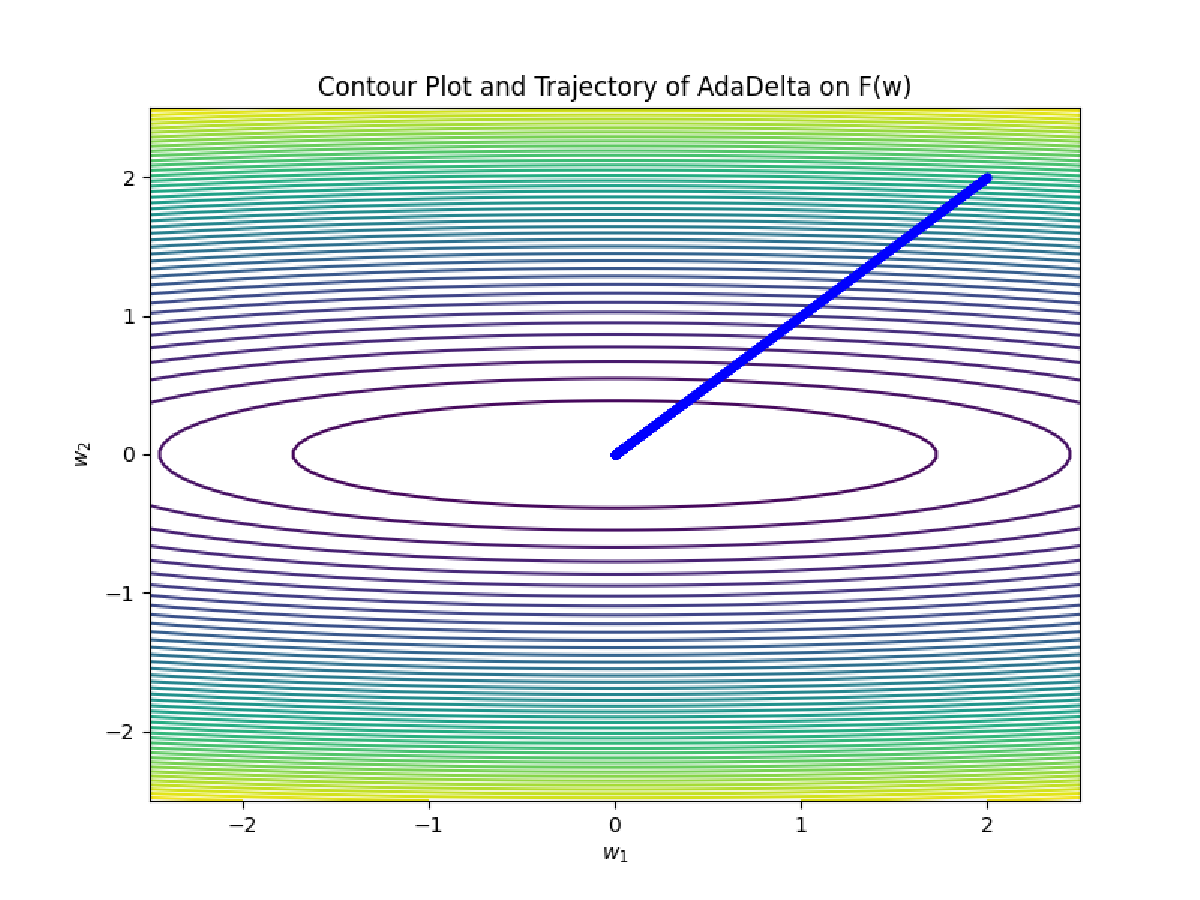
\includegraphics[width=.7\textwidth]{../Problem 8/ADADELTA_04.pdf}
	\caption{AdaDelta algorithm and trajectory with learning rate $\alpha=0.4$}
	\label{fig:lr=0.4}
\end{figure}
\vspace{2mm}

\subsection{Question B}
